\def\year{2021}\relax
%File: formatting-instructions-latex-2021.tex
%release 2021.1
\documentclass[letterpaper]{article} % DO NOT CHANGE THIS
\usepackage{aaai21}  % DO NOT CHANGE THIS
\usepackage{times}  % DO NOT CHANGE THIS
\usepackage{helvet} % DO NOT CHANGE THIS
\usepackage{courier}  % DO NOT CHANGE THIS
\usepackage[hyphens]{url}  % DO NOT CHANGE THIS
\usepackage{graphicx} % DO NOT CHANGE THIS

% ADJUSTED BY AFM ----------------------------------------------------------
\usepackage{amsmath} % ENTERED BY AFM

\urlstyle{rm} % DO NOT CHANGE THIS
\def\UrlFont{\rm}  % DO NOT CHANGE THIS
\usepackage{natbib}  % DO NOT CHANGE THIS AND DO NOT ADD ANY OPTIONS TO IT
\usepackage{caption} % DO NOT CHANGE THIS AND DO NOT ADD ANY OPTIONS TO IT
\frenchspacing  % DO NOT CHANGE THIS
\setlength{\pdfpagewidth}{8.5in}  % DO NOT CHANGE THIS
\setlength{\pdfpageheight}{11in}  % DO NOT CHANGE THIS
\nocopyright
%PDF Info Is REQUIRED.
% For /Author, add all authors within the parentheses, separated by commas. No accents or commands.
% For /Title, add Title in Mixed Case. No accents or commands. Retain the parentheses.
\pdfinfo{
/Title (ML Assignment 1)
/Author (Anthony Menninger)
/TemplateVersion (2021.1)
} %Leave this
% /Title ()
% Put your actual complete title (no codes, scripts, shortcuts, or LaTeX commands) within the parentheses in mixed case
% Leave the space between \Title and the beginning parenthesis alone
% /Author ()
% Put your actual complete list of authors (no codes, scripts, shortcuts, or LaTeX commands) within the parentheses in mixed case.
% Each author should be only by a comma. If the name contains accents, remove them. If there are any LaTeX commands,
% remove them.

% DISALLOWED PACKAGES
% \usepackage{authblk} -- This package is specifically forbidden
% \usepackage{balance} -- This package is specifically forbidden
% \usepackage{color (if used in text)
% \usepackage{CJK} -- This package is specifically forbidden
% \usepackage{float} -- This package is specifically forbidden
% \usepackage{flushend} -- This package is specifically forbidden
% \usepackage{fontenc} -- This package is specifically forbidden
% \usepackage{fullpage} -- This package is specifically forbidden
% \usepackage{geometry} -- This package is specifically forbidden
% \usepackage{grffile} -- This package is specifically forbidden
% \usepackage{hyperref} -- This package is specifically forbidden
% \usepackage{navigator} -- This package is specifically forbidden
% (or any other package that embeds links such as navigator or hyperref)
% \indentfirst} -- This package is specifically forbidden
% \layout} -- This package is specifically forbidden
% \multicol} -- This package is specifically forbidden
% \nameref} -- This package is specifically forbidden
% \usepackage{savetrees} -- This package is specifically forbidden
% \usepackage{setspace} -- This package is specifically forbidden
% \usepackage{stfloats} -- This package is specifically forbidden
% \usepackage{tabu} -- This package is specifically forbidden
% \usepackage{titlesec} -- This package is specifically forbidden
% \usepackage{tocbibind} -- This package is specifically forbidden
% \usepackage{ulem} -- This package is specifically forbidden
% \usepackage{wrapfig} -- This package is specifically forbidden
% DISALLOWED COMMANDS
% \nocopyright -- Your paper will not be published if you use this command
% \addtolength -- This command may not be used
% \balance -- This command may not be used
% \baselinestretch -- Your paper will not be published if you use this command
% \clearpage -- No page breaks of any kind may be used for the final version of your paper
% \columnsep -- This command may not be used
% \newpage -- No page breaks of any kind may be used for the final version of your paper
% \pagebreak -- No page breaks of any kind may be used for the final version of your paperr
% \pagestyle -- This command may not be used
% \tiny -- This is not an acceptable font size.
% \vspace{- -- No negative value may be used in proximity of a caption, figure, table, section, subsection, subsubsection, or reference
% \vskip{- -- No negative value may be used to alter spacing above or below a caption, figure, table, section, subsection, subsubsection, or reference

\setcounter{secnumdepth}{0} %May be changed to 1 or 2 if section numbers are desired.

% The file aaai21.sty is the style file for AAAI Press
% proceedings, working notes, and technical reports.
%

% Title

% Your title must be in mixed case, not sentence case.
% That means all verbs (including short verbs like be, is, using,and go),
% nouns, adverbs, adjectives should be capitalized, including both words in hyphenated terms, while
% articles, conjunctions, and prepositions are lower case unless they
% directly follow a colon or long dash


%Example, Single Author, ->> remove \iffalse,\fi and place them surrounding AAAI title to use it
\title{
Machine Learning - CS 7641
Assignment 2
	
}
\author {
    % Author
    Anthony Menninger \\
}

\affiliations{
    Georgia Tech OMSCS Program \\
    amenninger3\\
    tmenninger@gatech.edu

}

\begin{document}

\maketitle

\begin{abstract}
This paper first reviews three optimization problems using four different algorithms. The algorithms considered are Random Hill Climbing, Simulated Annealing, Genetic Algorithm and MIMIC.  The Four Peaks problem highlights Genetic Algorithm, the K Colors problem highlights MIMIC and the Knapsack Problem highlights Simulated Annealing.  The paper then reviews using Random Hill Climbing, Simulated Annealing, Genetic Algorithm for learning neural network weights for the MNIST image dataset and compares these results to using Back propagation.  
\end{abstract}

\section{Introduction}
The core library used in the experiments in this paper is mlrose [3].  This was developed by Georgia Tech students to support this class by providing a comprehensive tools set for reviewing randomized optimization.  I used the mlrose-hiive [2] fork, which has had other students fix bugs and enhance functionality.  All functions take a seed value which allows random functions to be repeated.  This was used and is documented in the code.

\section{Four Peaks and the Genetic Algorithm}
The Four Peaks problem is a simple problem, with fitness growing as consecutive 0's are added to the beginning of a bit string or consecutive 1's to the end.  In addition, there is a bonus if both the leading 0's and trailing 1's exceed a threshold.  This problem creates a very strong locality in the bit string, which will favor the Genetic Algorithms strength.  The problem was reviewed at 3 bit string sizes.   A length of 30 represents a state size of roughly 1 billion, a length of 60 a state size of 10 raised to the 18th, and a length of 90 a state size of 10 raised to the 27th power.  These are very large state spaces which effectively demonstrate the algorithms strengths. 

The Genetic Algorithm has two key parameters for optimization.  The population size is the number of active states that are considered in each iteration, where each iteration creates a new generation.  The new generation children are  created through combining parts of the bit strings of the previous generation parents with the highest fitness.  The second parameter is a mutation rate, which is a probability whether each bit in the children is randomly changed.  In this algorithm, exploration is created with crossover combinations and mutation and exploitation is governed by selecting only parents with the highest fitness.

\begin{figure}[htb]
\centering
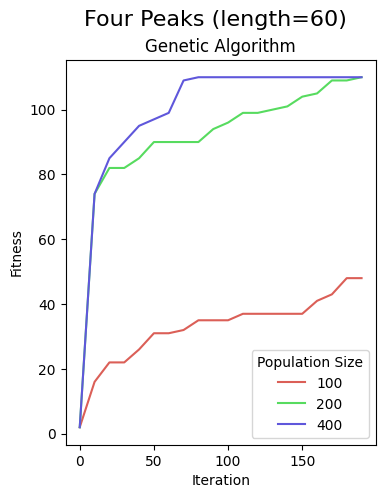
\includegraphics[width=2.75in, height=2.75in]{figures/Four_Peaks_length=60_Genetic_Algorithm_l_60_ma_60_p_100__200__400_mu_0.1_.png}
\caption{Four Peaks Genetic Algorithm:  This shows the fitness curves at different population sizes. Each iteration had a maximum of 60 attempts to find a better solution and a mutation rate of 0.1. }
\label{fig:four_peaks_ga}
\end{figure}

 \textbf{Figure \ref{fig:four_peaks_ga}} shows the Genetic Algorithm (GA) fitness curve at different population sizes for the Four Peaks problem.  Not surprisingly, the algorithm performs better with larger populations, where there are better chances for breeding successful children.  The algorithm was less sensitive to mutation rates for this problem, with 0.1 performing well, which was then used.

\begin{figure}[htb]
\centering
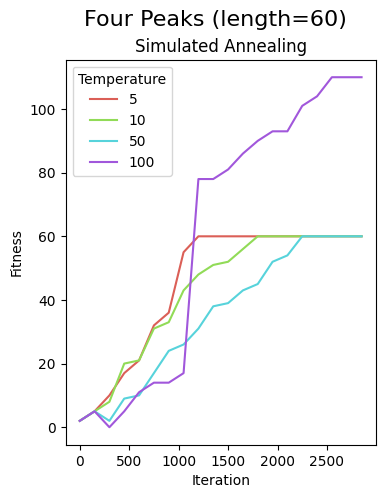
\includegraphics[width=2.75in, height=2.75in]{figures/Four_Peaks_length=60_Simulated_Annealing_l_60_ma_360_d_geom_t_5__10__50__100_.png}
\caption{Four Peaks Simulated Annealing:  This shows the fitness curves at different temperatures using a Geometric Decay schedule. Each iteration had a maximum of 60 attempts to find a better solution. }
\label{fig:four_peaks_sa}
\end{figure}

\textbf{Figure \ref{fig:four_peaks_sa}} shows the fitness curve for Simulated Annealing (SA) for different Temperatures.  The temperature governs how likely a candidate instance will be accepted during an iteration if it is not better than the current state instance.  This allows for exploration instead of only finding instances that are better, which is critical to avoid local maxima.    Higher temperatures allow for more exploration, which was necessary for SA to find reach maximum fitness for this problem.  Candidate neighbors are created by looking at local neighbors which only have one bit difference form the current instance.  Another key parameter is how the temperature is decayed in each iteration.  By slowly lowering the temperature, the algorithm is able to settle into the maximum basin instead of getting trapped in a local basin.  Three decay types considered with Geometric decay, Exponential Decay and Arithmetic Decay.  For this problem Geometric performed best at a length of 60 and was used.


\begin{figure}[htb]
\centering
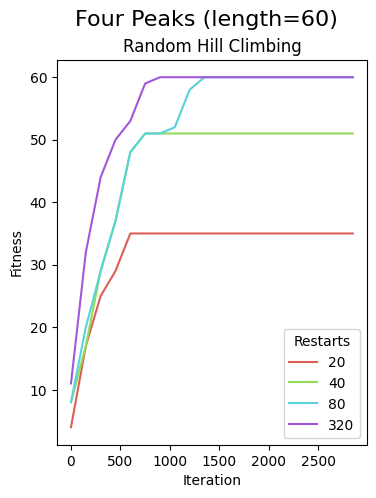
\includegraphics[width=2.75in, height=2.75in]{figures/Four_Peaks_length=60_Random_Hill_Climbing_l_60_ma_120_r_20__40__80__320_.png}
\caption{Four Peaks Random Hill Climbing: Each iteration had a maximum of 60 attempts to find a better solution. }
\label{fig:four_peaks_rhc}
\end{figure}


The Random Hill Climbing (RHC) algorithm looks at local candidate neighbors and at each iteration accepts the first reviewed with better fitness to the current instance.  If there is none better, it assumes this is a maximum.   A key parameter is the number of times the algorithm will restart from different random locations.   Its exploration is limited to the number of random restarts and the number of local neighbors.  It is considered greedy because it only accepts values that are better.

\textbf{Figure \ref{fig:four_peaks_sa}}  shows the results of Random Hill Climbing.  More restarts increases the chance of finding a better solution, but the maximum fitness values are significantly below those of the other algorithms reviewed.

\begin{figure}[htb]
\centering
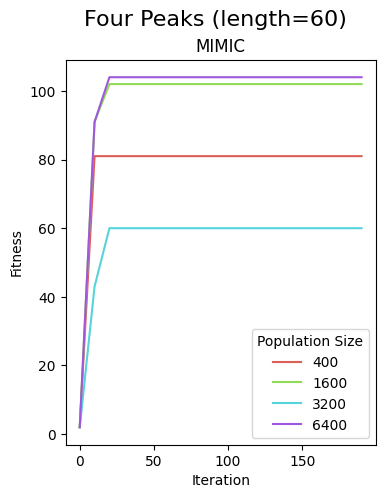
\includegraphics[width=2.75in, height=2.75in]{figures/Four_Peaks_length=60_MIMIC_l_60_ma_60_p_400__1600__3200__6400_k_0.1_.png}
\caption{Four Peaks MIMIC:  This shows the fitness curves at different population size. Each iteration had a maximum of 60 attempts to find a better solution. }
\label{fig:four_peaks_mimic}
\end{figure}

The MIMIC algorithm was created by Professor Isabell Charles.  It uses a population model to create a probability estimation that is refined through each iteration.  The goal is determine underlying structure in the problem through improving the distribution function.

\textbf{Figure \ref{fig:four_peaks_mimic}} shows the MIMIC results.  Like the GA, MIMIC uses a population size, keeping only the fittest in successive iterations.  The figure shows that a population size of 6400 performs best, but that 3200 performs the worst.  Another parameter is the top percentage to keep from one iteration to the next.  A Keep Percentage of 0.3 showed reduced performance, with 0.1 used for the population size reviews. 

\begin{figure}[htb]
\centering
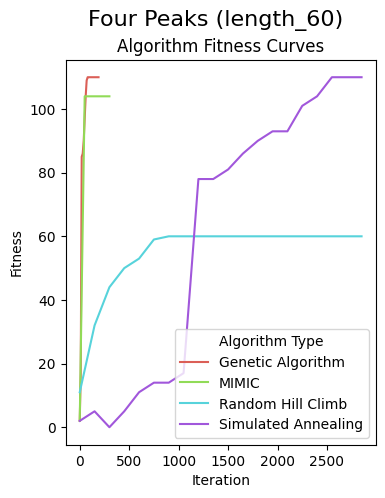
\includegraphics[width=2.75in, height=2.75in]{figures/Four_Peaks_length_60_Algorithm_Fitness_Curves_.png}
\caption{Four Peaks Fitness Comparisons: This shows the fitness curves of the different algorithms using the best tested settings at a bit string length of 60.  }
\label{fig:four_peaks_fitness_comparison_60}
\end{figure}

\begin{figure}[htb]
\centering
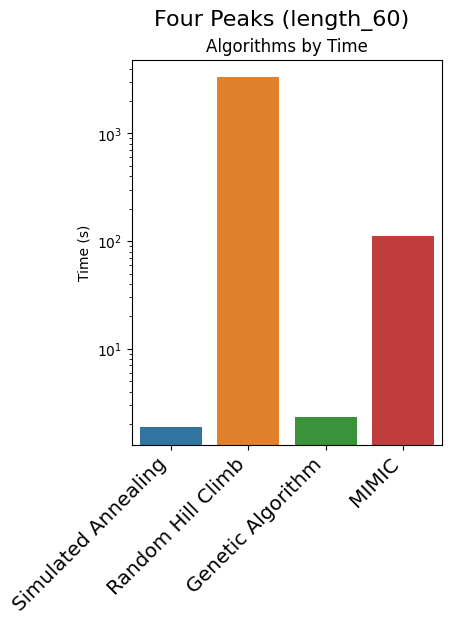
\includegraphics[width=2.75in, height=2.75in]{figures/Four_Peaks_length_60_Algorithms_by_Time_.png}
\caption{Four Peaks Wall Time Comparisons: This shows the time taken to reach the maximum fitness of the different algorithms using the best tested settings at a bit string length of 60.  }
\label{fig:four_peaks_walltime_comparison_60}
\end{figure}

In comparing them all, the Genetic Algorithm provided the maximum fitness in the least amount of iterations, as shown in \textbf{Figure \ref{fig:four_peaks_fitness_comparison_60}}.  This makes sense given the strong locality of the Four Peaks problem.  The MIMIC algorithm is close behind.  Simulated Annealing, which is using a hill climbing model with some exploration, is able to find a comparable solution, but it takes many more iterations.  Finally, Random Hill Climbing is not able to reach a comparable fitness level with only 320 restarts.

\textbf{Figure \ref{fig:four_peaks_walltime_comparison_60}} shows another measure of the algorithms, with the wall time to find the best solutions for each algorithm.  The Genetic Algorithm and Simulated Annealing are quick and roughly equivalent.  While MIMIC had few iterations, it took more than 20 times longer than GA or SA.  Pulling up the rear was Random Hill Climbing, which is slow due to the extended number of iterations it runs.

\section{Knapsack}

\section{K Colors}


\section{Neural Network Optimization}

The data set is The MNIST Database of Handwritten Digits [2].  This consists of instances of 28 X 28 greyscale images of the digits 0-9.  One transformation performed was that the values where scaled to 0 to 1, from 0 to 255.  For all but the neural network algorithm,  the images were flattened, creating 784 features, one for each pixel.  There are 60,000 training instances and 10,000 test instances.  I chose this because it is a good comparison to the first data set, with a very different type of data (images), which leads to significantly more features (784).  In addition, each of the features can be thought of as related to each other, as they are all positional in a two dimensional grid, while the first data set features do not have any necessary relation between themselves ie:  age is not related to sex.  

Did use Pytorch, run.  Switched over to mlrose


\section{References}
\begin{tabular}{l p{2.75in}}
\\
1 & The MNIST Database of Handwritten Digits. url: http://yann.lecun.com/exdb/mnist/.
\\
2 & Rollings, A. (2020). mlrose: Machine Learning, Randomized Optimization and SEarch package for Python, hiive extended remix. https://github.com/hiive/mlrose. Accessed: 2/11/2022
\\
3 & Hayes, G. (2019). mlrose: Machine Learning, Randomized Optimization and SEarch package for Python. https://github.com/gkhayes/mlrose. Accessed: 2/11/2022.
\\
4 & Menninger, A. (2022)  Code created for this experiment https://github.com/gkhayes/mlrose. Accessed: 2/11/2022.
\end{tabular}
\end{document}
